\section{D. Irga B. Naufal Fakhri (1174066)}
\subsection{Menulis Shapefile dengan PySHP}
\begin{enumerate}
	\item Nomor 1
	\lstinputlisting{src/tugas2/1174066/No1.py}
	\begin{figure}[H]
		
\includegraphics[width=6cm]{figures/Tugas2/1174066/No1.jpeg}
		\centering
		\caption{Point (Titik)}
	\end{figure}
	\item Nomor 2
	\lstinputlisting{src/tugas2/1174066/No2.py}
	\begin{figure}[H]
		
\includegraphics[width=6cm]{figures/Tugas2/1174066/No2.jpeg}
		\centering
		\caption{Point (Titik)}
	\end{figure}
	\item Nomor 3
	\lstinputlisting{src/tugas2/1174066/No3.py}
	\begin{figure}[H]
		
\includegraphics[width=6cm]{figures/Tugas2/1174066/No3.jpeg}
		\centering
		\caption{Point (Titik)}
	\end{figure}
	\item Nomor 4
	\lstinputlisting{src/tugas2/1174066/No4.py}
	\begin{figure}[H]
		
\includegraphics[width=6cm]{figures/Tugas2/1174066/No4.jpeg}
		\centering
		\caption{Point (Titik)}
	\end{figure}
	\item Nomor 5
	\lstinputlisting{src/tugas2/1174066/No5.py}
	\begin{figure}[H]
		
\includegraphics[width=6cm]{figures/Tugas2/1174066/No5.jpeg}
		\centering
		\caption{PolyLine (Garis)}
	\end{figure}
	\item Nomor 6
	\lstinputlisting{src/tugas2/1174066/No6.py}
	\begin{figure}[H]
		
\includegraphics[width=6cm]{figures/Tugas2/1174066/No6.jpeg}
		\centering
		\caption{Polygon (Bidang)}
	\end{figure}
	\item Nomor 7
	\lstinputlisting{src/tugas2/1174066/No7.py}
	\begin{figure}[H]
		
\includegraphics[width=6cm]{figures/Tugas2/1174066/No7.jpeg}
		\centering
		\caption{Polygon (Bidang)}
	\end{figure}
	\item Nomor 8
	\lstinputlisting{src/tugas2/1174066/No8.py}
	\begin{figure}[H]
		
\includegraphics[width=6cm]{figures/Tugas2/1174066/No8.jpeg}
		\centering
		\caption{Polygon (Bidang)}
	\end{figure}
	\item Nomor 9
	\lstinputlisting{src/tugas2/1174066/No9.py}
	\begin{figure}[H]
		
\includegraphics[width=6cm]{figures/Tugas2/1174066/No9.jpeg}
		\centering
		\caption{Polygon (Bidang)}
	\end{figure}
	\item Nomor 10
	\lstinputlisting{src/tugas2/1174066/No10.py}
	\begin{figure}[H]
		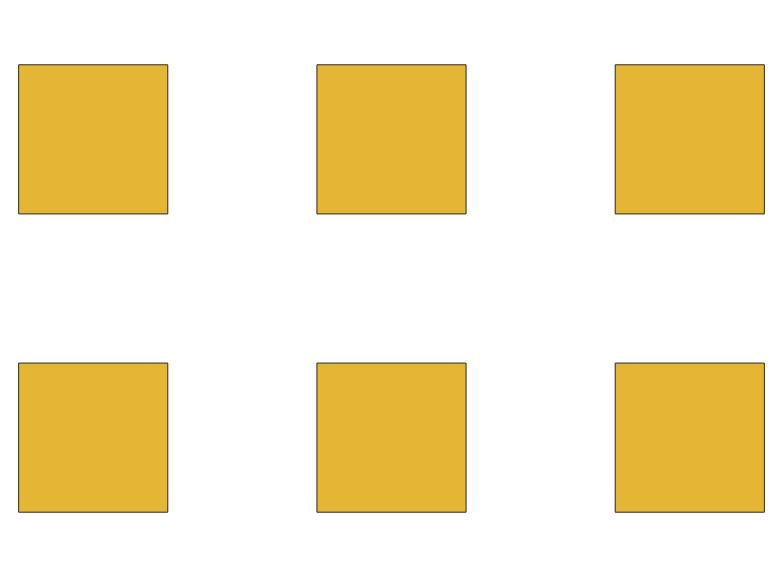
\includegraphics[width=6cm]{figures/Tugas2/1174066/No10.jpeg}
		\centering
		\caption{Polygon, Hasil modulus dari npm saya 1174066 adalah 2 jadi membuat bidang bujursangkar dan angka akhir dari npm saya adalah 6 jadi membuat bidangnya sebanyak 6}
	\end{figure}
\end{enumerate}
\subsection{Link}
https://youtu.be/k1zVCePA1Yg